\documentclass{deliverablereport}
\usepackage{pdfpages}

\deliverable{hpc}{pari-hpc2}
\deliverydate{2019-08-31}
\duedate{2019-08-31 (M48)}

\author{Bill Allombert, Karim Belabas}

\begin{document}
\maketitle
\githubissuedescription
\tableofcontents

\section{Introduction and rationale}

The \Pari library is a state-of-the-art library for number theory,
developed at Bordeaux University. It is an important component of the \Sage
computational system: \Sage uses it for example to implement number fields
and elliptic curves. \Pari itself is a C library but it comes with a
command-line interface called GP, and a GP-to-C compiler called GP2C.
Together, these form the software package \PariGP.

In experimental number theory, many large computations are embarassingly
parallel: no communication is needed between parallel tasks and there is
little data to pass from the main thread to the computing nodes. They usually
fit one of the following scenarii:
\begin{enumerate}
  \item exhaustive enumeration for theorem proving: for instance, asymptotic
    methods prove that all integers larger than some moderate bound $X$
    satisfy the theorem and we must check the remaining finitely many
    integers $n \leq X$. This generalizes to more complicated parameter sets
    as long as some theoretical proof leaves us with a finite
    moderately-sized space to enumerate.

  \item building databases: number theorists love building tables and
    databases of interesting objects, usually all (finitely many) objects
    of given ``kind'' and bounded ``size''. The motivation is for instance
    to infer general models from finite statistics or to test algorithms on
    large unbiased data sets. The $L$-functions and Modular Forms Database
    (LMFDB) is a prominent example.
    
  \item sampling: exploring a huge space until a favourable outcome occurs,
    e.g., a collision (as in the rho or ECM integer factoring method), or
    until sufficiently many data has been acquired to solve a problem by
    linear algebra (as in \emph{sieve} methods to factor integers or
    \emph{index calculus} algorithms to solve discrete logarithm problems).
    
  \item modular algorithms: where bounded integers are recognized by their
    congruence classes modulo sufficiently many primes and the Chinese
    Remainder Theorem (CRT), or interpolation algorithms where polynomials of
    bounded degrees are determined by sufficiently many values. The modular
    computations are independent of each other and offer a general speedup
    compared to a direct computation because they operate on much smaller 
    inputs and do not suffer from coefficient explosion.
\end{enumerate}

In all these cases, most of the computational effort is easily split into
independent parts of roughly equal sizes. In cases 3) and 4),
post-processing the independent results may be non trivial: integer
factorization and discrete logarithms end with a linear algebra problem in
huge dimensions; sophisticated quasi-linear time CRT or interpolation methods
are required for efficient modular reconstruction.

Now, typical number theorists have scant access to HPC clusters and use
personal machines. But even cheap laptops have 2 or 4 computing cores
nowadays. How to harness for \PariGP users that expected two-or fourfold
improvement ? And make that $N$-fold if an $N$-cores cluster becomes
available ? Of course, we also need to limit the implementation effort:
maintaining three or more variants of each algorithm (single core machine,
multicore single machine, cluster) is not manageable.

This deliverable, a merger of subtask D5.10 and demonstrator D5.16 in the
submitted proposal, was about implementing a generic parallel engine in the
\PariGP system, using it inside the system (expecting speed gains) and
exporting it for library users. Then releasing a \PariGP suite making those
improvements and new features available for the community, in particular
\Sage users and all softwares using the \Pari library.

More precisely, the MultiThread engine, or MT engine for short, transparently
supports: 1) sequential computation, 2) POSIX threads (for a single multicore
machine) and 3) Message Passing Interface (MPI, for clusters). It is usable
in two scenarii

\begin{itemize}
\item Explicit parallelism: the MT engine provides interfaces to launch
  subtasks in parallel and efficiently share global data with the tasks; the
  user must subdivide the tasks herself, handle load balancing and failures
  and recombine results, but she has complete control.

\item Implicit parallelism: a relevant selection of high-level system
  routines decide on their own to use explicit parallelism, or not. This is
  easier on the user but more complicated to handle, because there are many
  possible strategies and no automated algorithm can be optimal in all
  cases without some amount of user input: for instance, if routine $A$
  calls routine $B$ independently many times, it is easier and more efficient
  to parallelize $A$ and leave $B$ alone than to parallelize $B$. But how is
  the engine to know that $A$ is going to invoke $B$ many times ? Or that the
  calls to $B$ have roughly the same cost (or not, in which case load
  balancing becomes non trivial)?
\end{itemize}

\section{Work accomplished}
\subsection{Initial state at the start of the project}
Since PARI-2.7 (released 03/2014), it was already possible to build a
thread-safe PARI library, to use a handful of parallel GP control structures
(to enforce the Explicit scenario in the previous section) and to use the
standard POSIX threads interface in separate autonomous C programs.

\subsection{The generic MT engine}
The MT engine was written and finalized in 2015 and 2016 and is in
production since PARI-2.9 (released 11/2016), it supports sequential
evaluation (no parallelism), POSIX threads and MPI within the same code
base. The full suite is supported: GP2C correctly compiles GP code which is
making use of the GP parallel interface.

Since then, the engine has been extensively tested on Unix/Linux
desktop computers (up to 96 cores) and clusters (up to 128 nodes), and on
laptops running Linux, OSX and Windows 10 (Bash on Windows). As expected, in
embarassingly parallel algorithms, the measured speedup was essentially
linear in the number of available cores; in more complicated programs where
post-processing is not negligible, the gain is less important.

User documentation for the engine is included in an annex at the end of the
present document.

\subsection{Using the MT engine throughout the PARI library}
Development work since PARI-2.9 has been targetted at using the MT engine
wherever it made sense in the \Pari code base, after a preliminary assessment
in early 2017: we strived to implement them by order of decreasing impact
inside the \Pari library and by increasing complexity of existing sequential
code. In particular, basic routines with multiple applications were attempted
first, before the higher level ones. In the current public release
(PARI-2.12, released 06/2019), the following functions are covered by the
engine:

\begin{itemize}
\item simultaneous Chinese remaindering (CRT) problems for a fixed set of
  moduli; a fast (quasi-linear time) sequential CRT routine was actually
  written as the engine was developped (previous CRT implementation was
  quadratic instead of linear). This a building block used to recognize
  matrices or polynomials with huge rational coefficients, used in standard
  modular algorithms, e.g., polynomial gcd, characteristic polynomial,
  inverses of algebraic number; inverse or determinant of matrix.

\item fast linear algebra over the rationals and cyclotomic fields; this 
  uses intensively a new implementation of fast CUP decomposition (in time
  $O(\text{dim}^{\log_2 7})$) over finite fields developped by Peter Bruin
  (2018) and turned into a general linear algebra package by Bill Allombert;
  this is a critical building block for the Modular Forms and Modular symbols
  packages.

\item polynomial resultant in $\mathbb{Z}[X] \times \mathbb{Z}[X,Y]$
  via Chinese remainders and Lagrange interpolation; this operation is a
  building block for algebraic number theory computations over number
  fields (compositum, relative extension, norm, characteristic polynomial).

\item computation of classical modular polynomials for about 20 invariants
  (elliptic $j$, Weber $f,f_1,f_2$ functions, small eta quotients, \dots);
    this is a building block for complex multiplication and many algorithms
    exploiting isogenies between elliptic curves (SEA point-counting
    algorithm, ECPP primality test, supersingularity test).

\item discrete logarithm over finite fields (prime fields and
  $\mathbb{F}_{p^e}$ for word\item sized prime p);

\item APRCL primality proof;

\item Fourier coefficients of $L$-functions (Hasse-Weil function for
  elliptic curves over number fields, symetric powers of elliptic cuves or
  curves of genus 2 over $\mathbb{Q}$; Artin $L$-functions of Galois
  representations).
\end{itemize}

For the first two items, new sequential code (fast CRT and multimodular
reduction) was developped specifically, in order to maximize the effect of
the MT engine by making both the parallel modular tasks (executed
sequentially on each node/thread) and the pre- and post-processing
(resp.~reduction and CRT) as efficient as possible.

In the other cases, compared to the pre-existing sequential code, the
parallel version adds about 15 extra lines of C on average, conveniently
encapsulated in a separate \texttt{worker} object (see Annex's chapter 3).
Since the engine takes care of most usual pitfalls of parallel programming,
e.g. concurrent access or deadlocks, the modifications are routine
\emph{provided} 1) the original sequential code is free of side effects and
well understood; 2) the code contains natural splitting or synchronization
points.

Condition 1) was not always satisfied and we took the opportunity to simplify
and rewrite existing code in order to improve the code quality before adding
parallel instructions. Condition 2) was usually satisfied; one exception was
modular computations in a dynamic setting, where we want to stop as soon as
the result can be ``recognized'' and we do not know in advance how many
modular threads will be needed. In that case, the behaviour very much depends
on the size of the result, which can be bounded in advance, but possibly
pessimistically. We handled that case with a naive doubling strategy: we
double the number of modular threads until the result is obtained; this way
we spend at most double the time which would be needed, had we known the
result size in advance.

\subsection{Impact and Related work}

In this section we limit ourselves to a few representative applications
for the functions listed in the previous one.

The fast linear algebra over the rationals is a major component
of the ``Modular Symbols'' package (developped between 2013 and 2018
by Karim Belabas and Bernadette Perrin-Riou, released in two stages: PARI-2.9
(2016) and PARI 2.11 (2018)): modular symbols are a standard way to work with
spaces of classical modular forms $M_k(\Gamma_0(N))$ using
$\mathbb{Q}$-linear algebra. The linear algebra improvements allowed to write
routines such as the \kbd{ellweilcurve} GP function, which computes the
strong Weil curve in an isogeny class of rational elliptic curves starting
from the modular eigensymbol having the same eigenvalues of the newform
attached to the isogeny class (by the modularity theorem of Wiles at al.) In
the range of the Cremona tables that we wanted to check (conductor $N \leq
500,000$), this requires computing kernels of rational matrices of dimension
up to $N / 6\approx 83,333$.

The fast linear algebra over cyclotomic fields is a critical component of the
new ``Modular Forms'' package (developped between 2016 and 2018 by Bill
Allombert, Karim Belabas and Henri Cohen, released in PARI-2.11): to handle
classical spaces of modular forms $M_k(\Gamma_0(N), \chi)$, this package
requires working with large matrices (of dimension $\Omega(kN)$) over the
cyclotomic field $\mathbb{Q}(\chi)$. In fact, the extension of linear algebra
from the rationals to cyclotomic fields was motivated by this single (major)
application.

The fast computation of modular polynomials allowed Jared Asuncion to
implement the ECPP primality proof in full generality, without relying on the
presence of precomputed tables, which would have limited the size of the
primes the implementation could handle. For the same reason, the Satoh point
counting algorithm for elliptic curves over large non-prime finite fields
could be implemented in full generality by Bill Allombert. Both algorithms
are now part of the \PariGP system.

The parallel computation of Fourier coefficients is used
in the ``$L$-functions'' package, which computes values of motivic
$L$-functions $L_f(s) = \sum_{n>0} a(n,f) n^{-s}$ at complex points $s\in
\CM$, where $f$ is some ``motive'' of geometric origin, for instance a
modular form or a curve defined over some number field. For given $f$, this
requires computing all Fourier coefficients $a(n,f)$, $n \leq B$, for
some large bound $B$ depending moderately on $s$ (which allows for
precomputations if all required $s$ belong to the same region, e.g., a
bounded rectangle in the critical strip). For simple $L$-functions, the
$a(n,f)$ are easy to compute and not worth the overhead of the MT engine; for
instance, if $L_f$ is the Riemann zeta function $\zeta$, then $a(n,f) = 1$
for all $n$. We have written a generic wrapper valid for all $L$ functions
satisfying an Euler product that computes the required $a(n,f)$ from the
$a(p^k,f)$, where $p$ is now a prime number and $p^k\leq B$. The computations
for different primes $p$ are independent and are now made in parallel for all
complicated $L$-functions. The attached generic speedup applies to all
$L$-function related code.

\subsection{Work in progress}

We have rewritten \Pari's Multiple Polynomial Quadratic Sieve (MPQS) integer
factorization sequential implementation so as to allow its parallelization:
this was a daunting task since the existing implementation was both efficient
and complicated, full of side effects (modifying global state, writing
to/reading from files); so this particular application was attempted last.
The rewrite was completed at the beginning of August 2019 in the public
\kbd{master} git branch, the parallel variant will be written in Autumn 2019.
This is work in progress.

The existing class group and units implementation is an equally difficult
case with a code base developped over 25 years by many people. After our 2017
assessment, we decided against modifying it during the course of the
OpenDreamKit projet: in most applications we inventoried, a single class
group computation (made ten time faster, say, by internal parallel
computations) would not make a major difference. Naive external
parallelization appeared sufficient, where we handle $N$ similar class group 
and unit computations in parallel instead of parallelizing each single
instance to try and make it $N$ times faster. This application may be
considered later but is not a high-priority task.

\subsection{Dissemination}

Activities were organized around parallel computation in \PariGP
at the following OpenDreamKit conferences:
\begin{itemize}
  \item Atelier \PariGP 2016 (Grenoble) \emph{Parallel PARI with GP2C},
  1h20 tutorial by Bill Allombert.
  \item Atelier \PariGP 2017 (Lyon) and \PariGP 2018 (Besançon)
  crashtest of MT engine: all participants compiled their own \Pari library and
  GP/GP2C  binaries at the start of the Atelier, without altering their
  workflow or existing programs except by enabling the MT engine via
  \texttt{Configure --mt=pthread}. No configuration problems arose and this
  transparently yielded the expected speedups for all multicore laptops during
  the week.

  \item Atelier \PariGP 2019 (Bordeaux) \emph{Parallel GP programming},
  1h20 tutorial by Bill Allombert.
\end{itemize}
The various Ateliers were also the most important way we got feedback from
users about the proposed interfaces and features.


\section{Examples}
TODO

\begin{verbatim} % single
? parapply(factor, [2^i - 1 | i <- [1..201]]);
time = 4,933 ms.

\\ random degree 1000 polynomials with 1000-bit coefficients
? a = random(2^1000 * 'X^1000); \
  b = random(2^1000 * 'X^1000); \
  c = random(2^1000 * 'X^1000); P = a*b; Q = a*c;
? gcd(P, Q)

\\ random dim 300 square matrix with 100-bit coefficients
? M = matrix(300,300, i,j, random(2^100)); M^(-1);
? gcd(P, Q)
\end{verbatim}

\begin{verbatim}
? default(nbthreads, 16)
? parapply(factor, [2^i - 1 | i <- [1..201]]);
cpu time = 6,773 ms, real time = 1,561 ms.
? default(nbthreads, 2)
? parapply(factor, [2^i - 1 | i <- [1..201]]);
cpu time = 5,112 ms, real time = 2,607 ms.
\end{verbatim}

\begin{verbatim}
In [1]: from cypari2 import Pari; pari = Pari()

In [2]: pari.default("nbthreads", 2)

In [3]: L = [2**i - 1 for i in range(1, 201)]

In [4]: %time res = pari.parapply("factor", L)
CPU times: user 6.76 s, sys: 170 ms, total: 6.93 s
Wall time: 3.6 s
\end{verbatim}

\appendix

\section{Snapshot of the documentation at the time of delivery}

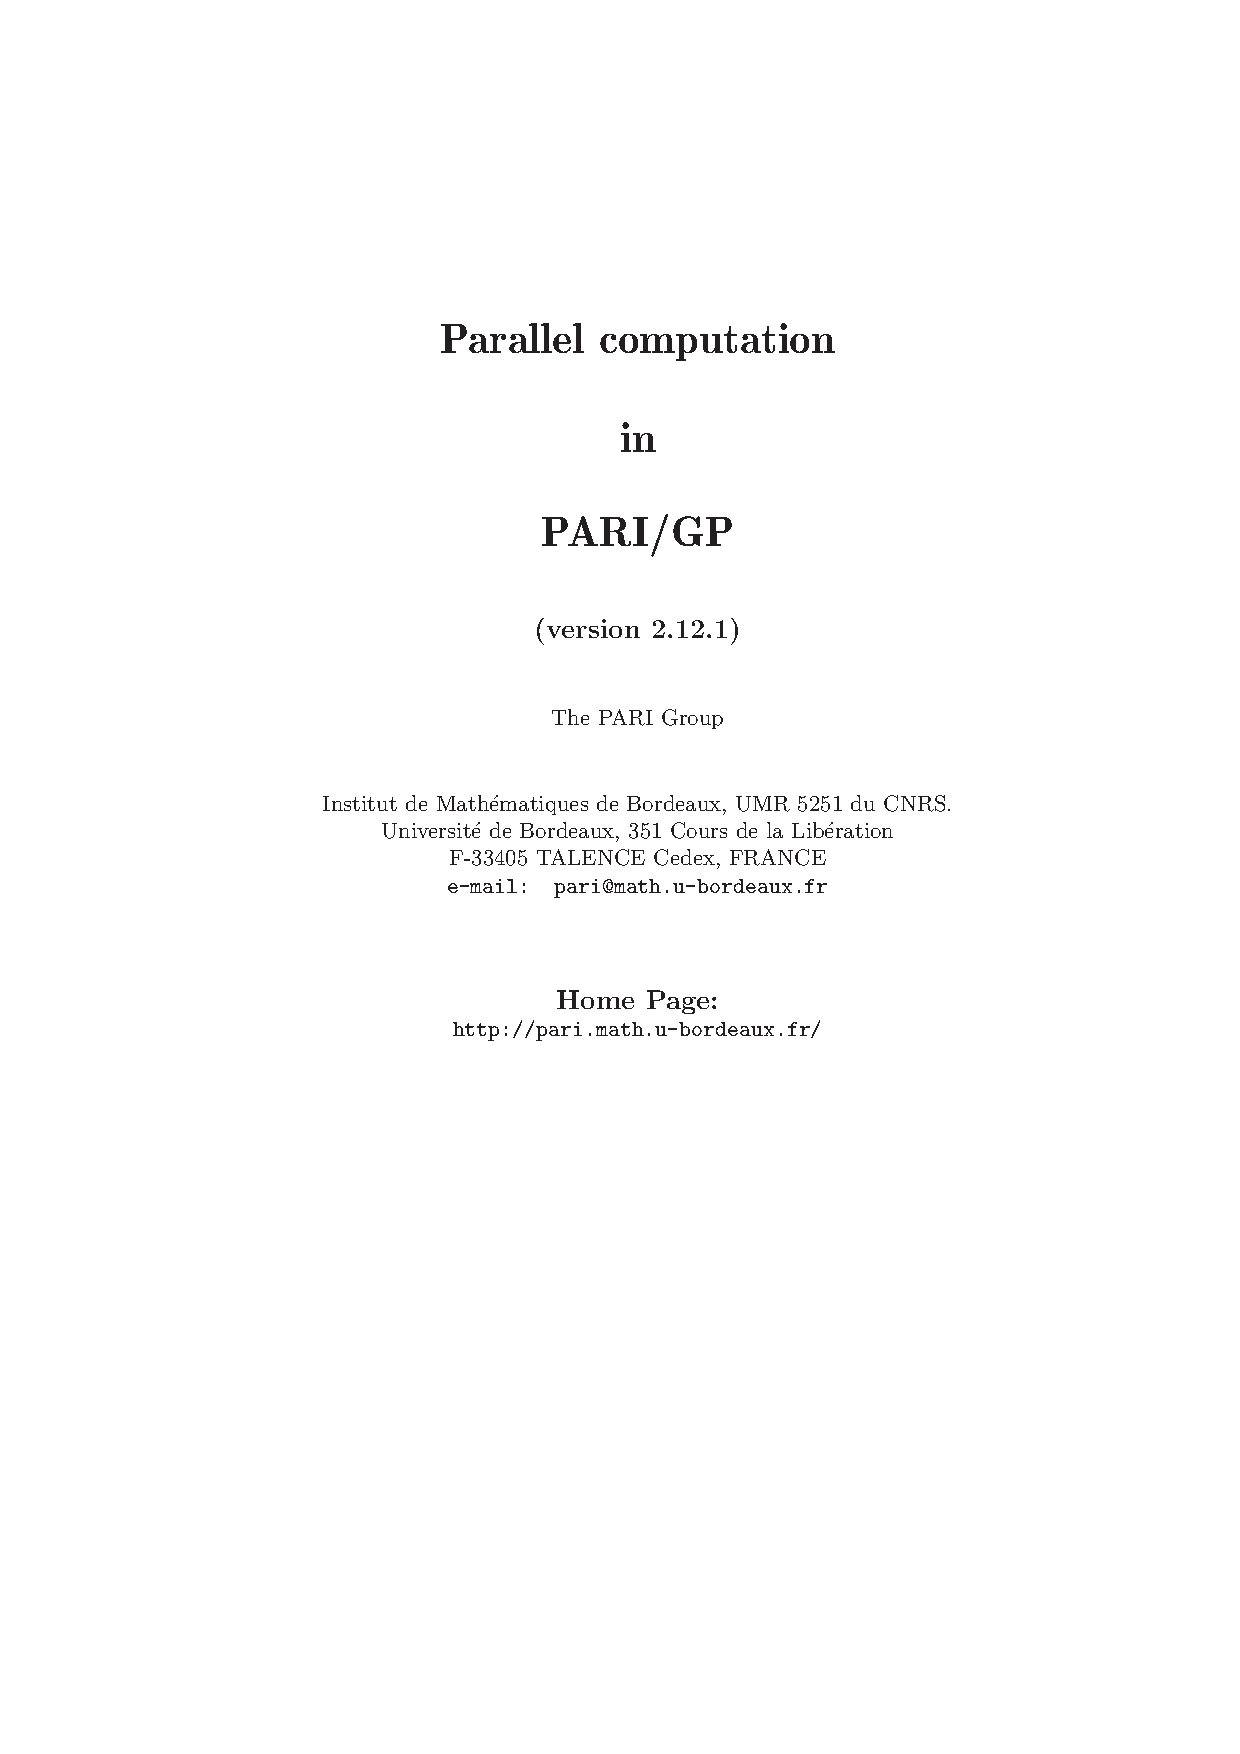
\includepdf[pages=-]{ODK-parallel.pdf}
\end{document}
